\documentclass[../../e3_tp3_main.tex]{subfiles}

\begin{document}




%capítulo
\chapter{Ejercicio 2}



The inputs of the system are $A$, which feeds the FSM with the sequence 1-1-0-1 sequentially and $B$ which corresponds to the current bit of the sequence to compare. To create the sequential flow of $A$, 1-1-0-1 can be loaded in parallel to a shift register and then be shifted. A new auxiliary input $W$ which is simply an XOR of $A$ an $B$, so $W=0$ if $A=B$ and $W=1$ otherwise. This helps reduce the complexity of both FSM.

The output is $Z=1$ if the sequence has been detected in the last clock cycle, and $Z=0$ otherwise.

When a conclusion is reached (ie. when the input sequence is found to be the same as 1-1-0-1 or different) the FSM jumps to its first state.

\section{Moore-type FSM implementation}
\subsection{FSM flow-chart}
\begin{equation}
	\tikzfig{moore_machine}
\end{equation}

\subsection{State descriptions}
\begin{table}[H]	%moore state descriptions
	\centering
		\begin{tabular}{|c|c|c|c|}
		\hline 
		$y_0,y_1,y_2$ & State name & Description & Z \\ 
		\hline 
		000 & 0 MATCH & No bits were matched & 0\\ 
		\hline 
		001 & 1 MATCH & Only one bit was matched & 0\\ 
		\hline 
		011 & 2 MATCH & Only two bits were matched & 0\\ 
		\hline 
		010 & 3 MATCH & Only three bits were matched & 0\\ 
		\hline 
		110 & 4 MATCH & The whole sequence has been matched & 1\\ 
		\hline 
		\end{tabular} 
	\caption{Possible states for the Moore-type FSM implementation.}
	\label{tab:ej2_moore_states}
\end{table}


\subsection{State transition table}

\begin{table}[H]	%moore state descriptions
	\centering
	\begin{tabular}{|c|c|c|c|}
	\hline 
	$y_0,y_1,y_2$/ W & 0 & 1 & output\\ 
	\hline 
	000 & 001 & 000 & 0\\ 
	\hline 
	001 & 011 & 000 & 0\\ 
	\hline 
	011 & 010 & 000 & 0\\ 
	\hline 
	010 & 110 & 000 & 0\\ 
	\hline 
	110 & 001 & 000 & 1\\ 
	\hline 
	\end{tabular} 
	\caption{Possible states for the Moore-type FSM implementation.}
	\label{tab:ej3_moore_states}
\end{table}


\subsection{Outputs and next states Karnaugh maps}
\begin{figure}[H]
	\centering
	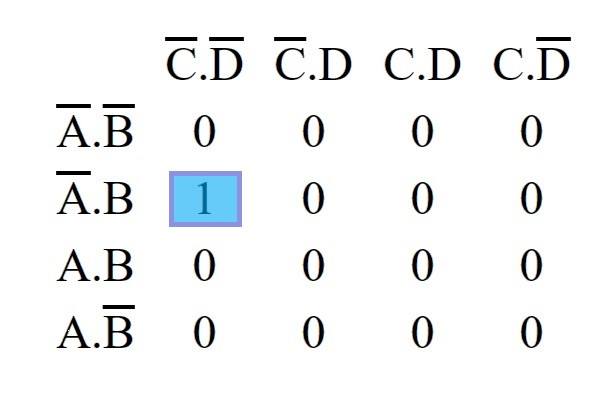
\includegraphics[scale=0.65]{figures/e3_tp3_ej2_moore_y0_kmap.jpg}
	\caption{$Y_0$ Karnaugh map}
\end{figure}

\begin{figure}[H]
	\centering
	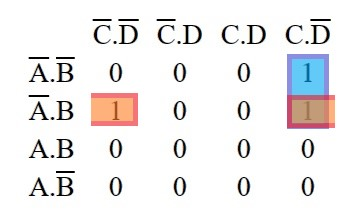
\includegraphics[scale=1]{figures/e3_tp3_ej2_moore_y1_kmap.jpg}
	\caption{$Y_1$ Karnaugh map}
\end{figure}

\begin{figure}[H]
	\centering
	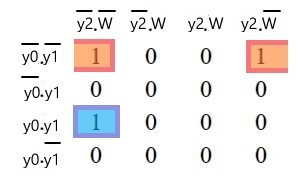
\includegraphics[scale=1]{figures/e3_tp3_ej2_moore_z_kmap.jpg}
	\caption{$Z$ Karnaugh map}
\end{figure}


\subsection{Outputs and next states schematics}
%schematics as sum-of-products


\section{Mealy-type FSM implementation}
\subsection{FSM flow-chart}
\begin{equation}
	\tikzfig{mealy_machine}
\end{equation}


\subsection{State descriptions}
\begin{table}[H]	%moore state descriptions
	\centering
		\begin{tabular}{|c|c|c|c|}
		\hline 
		$y_0,y_1$ & State name & Description \\ 
		\hline 
		00 & 0 MATCH & No bits were matched \\ 
		\hline 
		01 & 1 MATCH & Only one bit was matched\\ 
		\hline 
		11 & 2 MATCH & Only two bits were matched\\ 
		\hline 
		10 & 3 MATCH & Only three bits were matched \\ 
		\hline
		\end{tabular} 
	\caption{Possible states for the Moore-type FSM implementation. Note: when the sequence has been found, the FSM transitions from 3 MATCH to 0 MATCH.}
	\label{tab:ej2_mealy_states}
\end{table}



\subsection{State transition table}

\begin{table}[H]	%moore state transitions
	\centering
		\begin{tabular}{|c|c|c|}
		\hline 
		$y_0,y_1$/W & 0 & 1 \\ 
		\hline 
		00 & 01/0 & 00/0 \\ 
		\hline 
		01 & 11/0 & 00/0 \\ 
		\hline 
		11 & 10/0 & 00/0 \\ 
		\hline 
		10 & 00/1 & 00/0 \\ 
		\hline 
		\end{tabular} 
	\caption{Possible states for the Mealy-type FSM implementation.}
	\label{tab:ej2_mealy_state_transitions}
\end{table}


\subsection{Outputs and next states Karnaugh maps}
\begin{figure}[H]
	\centering
	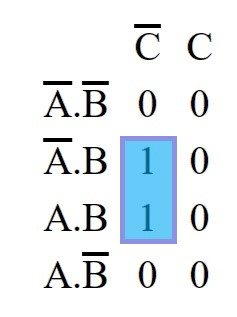
\includegraphics[scale=1]{figures/e3_tp3_ej2_mealy_y0_kmap.jpg}
	\caption{$Y_0$ Karnaugh map}
\end{figure}

\begin{figure}[H]
	\centering
	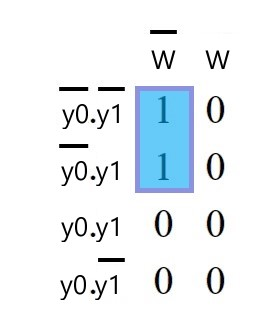
\includegraphics[scale=1]{figures/e3_tp3_ej2_mealy_y1_kmap.jpg}
	\caption{$Y_1$ Karnaugh map}
\end{figure}

\begin{figure}[H]
	\centering
	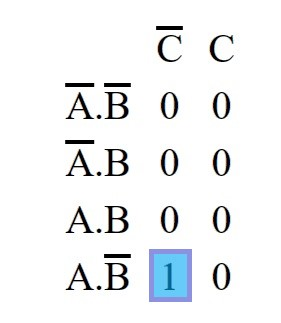
\includegraphics[scale=0.9]{figures/e3_tp3_ej2_mealy_z_kmap.jpg}
	\caption{$Z$ Karnaugh map}
\end{figure}

\subsection{Output and next states schematics}
%schematics as sum-of-products



\end{document}
